\chapter{Mobility Patterns}

Mobility patterns are an abstraction of the movement of individuals or groups of individuals that show their cumulative behaviour. They can be divided into \textbf{global patterns}, which describe the movement of sets of individuals, and \textbf{local patterns}, which refer to the movement of a single individual. This chapter will show various methods to extract both types of patterns from mobility data.

\section{Global Patterns}

A simple way to extract global patterns is to use a clustering algorithm on trajectory data. However, the choice of clustering algorithm and distance measure is crucial, since trajectories cannot be treated as regular tabular data. Also, interpreting clusters as patterns is not immediate: if we, for example, ran k-means on a trajectory dataset, would the centroids of the clusters represent meaningful patterns?

\subsection{Distances}
First, let's look at some distance measures. Trajectory distances can be divided in three categories, depending on how the trajectories themselves are treated:
\begin{itemize}
    \item Those who treat trajectories as \textbf{sets} of points, such as Hausdorff distance;
    \item Those who treat trajectories as \textbf{sequences} of points, such as Fréchet distance;
    \item Those who treat trajectories as \textbf{time-stamped sequences} of points, such as the Average Euclidean distance.
\end{itemize}

\paragraph{As sets} 
Two distances of this type are \textbf{common destination} and \textbf{common origin} distances, which both reduce a trajectory to its end/start point, respectively. The distance between a pair of trajectories is defined as the distance (e.g., Euclidean) between their end/start point only.
\begin{figure}[h]
    \vspace{10pt}
    \centering
    \includesvg[width=0.5\textwidth]{img/dist_common.svg}
    \caption{Common origin vs Common destination distances.}
\end{figure}

\textbf{Hausdorff distance} measures the maximum distance of all distance values from a point of one trajectory $T_1$ to the nearest in another trajectory $T_2$. Another way to interpret Hausdorff distance is to consider it the smallest buffer to build around $T_1$ to include all points of $T_2$.
\begin{align*}
    &\text{Hausdorff}(T_1, T_2) = \sup_{i} \inf_j d(T_1(i), T_2(j)) \\
    &\text{symm. Hausdorff}(T_1, T_2) = \max \{\sup_{i} \inf_{j} d(T_{1}(i), T_{2}(j)), \sup_{j} \inf_{i} d(T_{1}(i), T_{2}(j)) \}
\end{align*}
However, when applied to trajectories, Hausdorff can yield counter-intuitive results; for example, when the points of the two trajectories are spatially close to each other, but they make different detours, such as in the figure below.
\begin{figure}[h]
    \centering
    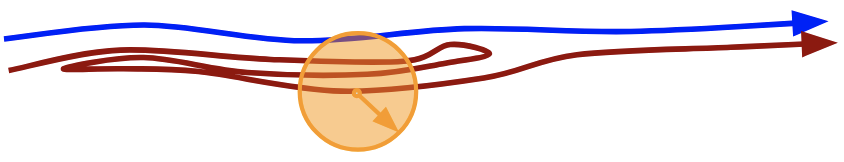
\includegraphics[width=0.5\textwidth]{img/dist_haus.png}
    \caption{Hausdorff distance between two trajectories, visualized in orange. Even though they are very different, their distance is misleadingly small.}
\end{figure} 

\paragraph{As sequences}
\textbf{Frèchet distance} can be seen as the equivalent of Dynamic Time Warping but applied to continuous curves. Formally, it is calculated as:
\begin{equation*}
    \text{Frechet}(T_1, T_2) = \inf_{\alpha, \beta} \max_{t \in [0,1]} \{ d(T_1(\alpha(t)), T_2(\beta(t)))\}
\end{equation*}
where $\alpha, \beta$ are non-decreasing mappings from $[0,1]$ to the points along $T_1$ and $T_2$ in forward order. In other words, it takes in consideration the direction of the trajectories, and in which order their points appear in each. Dynamic Time Warping and Edit Distance with real values can also be used on trajectories. It is important to note that most of these methods assume constant sampling rates.

\paragraph{As time-stamped sequences}
\textbf{Average Euclidean distance} transforms trajectories into continuous spatio-temporal curves via linear interpolation of pairs of subsequent points. The distance between two trajectories is calculated as:
\begin{equation*}
    D(T_1, T_2)|_T = \frac{\int_T d(T_1(t), T_2(t)) dt}{|T|}
\end{equation*}
where $T$ is the time interval over which the trajectories have been recorded. This distance only considers pairs of contemporary points, and does not use any matching/shifting of subsequences to align the two trajectories.

\subsection{Algorithms}
In principle, any distance-based clustering can be used, with the following requirements: it must be able to identify non-globular clusters, it must tolerate noisy data, it must be computationally cheap, and can be applied to structured data. A common choice is to use density-based clustering algorithms such as DBSCAN or OPTICS. These algorithms label points as either core points (on the inside of a cluster), border points (on the edge of a cluster), or noise points (not belonging to any cluster) on the basis of two hyperparameters, \textit{eps} and \textit{minPts}. A core point has \textit{minPts} points within \textit{eps} distance, a border point in whithin \textit{eps} distance to a core one but has less than \textit{minPts} points in its neighborhood, and finally noise points are those who are too far away to be connected to any core point. After the labeling, clusters can be formed by connecting core points and border points close to each other in a single cluster.

\section{Local Patterns}
A simple way to extract local patterns is to transform the trajectories in the dataset to a sequence of areas, building a tessellation over the area of interest and assigning each point of a trajectory to the area it falls in; the resulting sequences can be then used as input for sequential pattern mining algorithms that will identify frequent subsequences. The results are influenced by how the tessellation is constructed and how fine it is.

\textbf{Trajectory flocks} are groups of objects that move together close to each other for a certain time interval. A flock can be formally defined as follows: given a set of $n$ trajectories of entities, a flock in a time interval $I$, whose is at least $k$, consists of at least $m$ entities such that for every point in time $t \in I$ there is a disk of radius $r$ that contains all $m$ entities. $m$, $k$, and $r$ are hyperparameters that can be tuned to control how flocks are extracted.

\textbf{Convoys} are similar to flocks, but to count as a convoy, entities must be density-connected. Formally: given a set of trajectories of entities, a distance threshold $r$, a time threshold $k$, and a size $m$, a convoy is a set of $m$ entities that are found to be density-connected for at least $k$ consecutive time points w.r.t. $r$ and $m$. Convoys can capture groups of connected entities of irregular shapes. \textbf{Swarms} are defined similarly to convoys, but do not require the entities to appear in $k$ consecutive time points: the total number of times in which the entities are connected must be at least $k$, but an entity may disappear for a few time points and then reunite with the rest while still counting as part of the swarm.
\begin{figure}[h]
    \centering
    \includesvg[width=0.85\textwidth]{img/flock_convoy_swarm.svg}
    \caption{Differences between flocks, convoys, and swarms.}
\end{figure}


A \textbf{moving cluster} is yet another type of local pattern, which does not require the entities in it to be the same from start to finish. Let $H = \{t_1, t_2, \dots t_n\}$ be a timestamped history, and $S = \{o_1, o_2, \dots o_m\}$ a collection of objects that have moved during $H$, each with a variable lifetime. A snapshot $S_i$ of $H$ is the set of objects and their locations that exist at time $t_i$. Clusters of density-connected entities can be found at each snapshot. Let $g = c_1, c_2, \dots, c_k$ be a sequence of snapshot clusters such that the timestamp of $c_i$ is exactly before that of $c_{i+1}$; then $g$ is a moving cluster w.r.t. to a threshold $\theta$ ($0 < \theta \leq 1$) if:
\begin{equation*}
    \text{Jaccard}(c_i, c_{i+1}) = \frac{|c_i \cap c_{i+1}|}{|c_{i} \cup c_{i+1}|} \geq \theta, \quad \forall 1 < i \leq k
\end{equation*}
This means that as long as the Jaccard coefficient is high enough between every two consecutive shanpshots, the cluster is considered a pattern, and entities can move in and out of it.

In practice, the algorithm used to find moving clusters scans through each snapshot and runs DBSCAN/OPTICS on the entities in that snapshot, identifying clusters. At each step, a set $\mathcal{G}$ is used to keep track of current moving clusters, so that the clusters found in the current snapshot can be compared to the existing ones. If a moving cluster in $\mathcal{G}$ is extended by some new cluster, the two are merged and added to $\mathcal{G}_{new}$. If an existing moving cluster is not extended by any cluster, it is outputted. Any new cluster that does not extend any old moving cluster is also added to $\mathcal{G}_{new}$, as it may be the start of a new moving cluster. Finally, $\mathcal{G}$ is replaced by $\mathcal{G}_{new}$ and the process is repeated for the next snapshot.

\textbf{Trajectory patterns}, or \textbf{T-patterns}, are sequences of regions frequently visited in a specific order and with similar transition times. A T-pattern is defined as a pair $(S,A)$, where $S = \langle (x_0, y_0), \dots, (x_k, y_k) \rangle$ is a sequence of points in $R^2$, and $A = \langle \alpha_1, \dots, \alpha_k \rangle \in R^k_+$ is the temporal annotation of the sequence. A T-pattern is frequent if it has support higher than some threshold $s_{min}$, where the support is calculated as the number of input trajectories that ``spatio-temporally'' contain the pattern. Containment does not require spatial or temporal data to perfectly match between the pattern and the input sequence to contribute to the support. Temporal containment requires that each element of the pattern is contained in an element of the sequence in the same order they appear, and that the time annotation between each pair of subsequent elements is similar for both the pattern and the sequence (the difference should be less than some threshold $\tau$). Spatial containment requires that all the points of the pattern are contained, in order, in neighborhoods of points of the sequence.

Trajectories can also be treated as sequences of \textbf{regions of interest}, so that spatial information can be discarded after a preprocessing phase that assigns each pair of coordinates in the dataset to a RoI. If RoIs are not known a priori, they may be automatically identified by analyzing the dataset to find the most visited areas and/or using information found in external datasets.

\section{Deep Learning for Trajectory Clustering}
Recent approaches use deep learning models to facilitate detection and analysis of mobility patterns. A model can be trained to produce embeddings of trajectiories, automatically learning the best representation to capture similarity and differences between them, producing a clustering over this latent space. An example of such framework is \textbf{Deep Embedded TrajEctory ClusTering network} (\textbf{DETECT}). It operates in three parts:
\begin{enumerate}
    \item First, it summarizes the critical parts of the trajectories, and augments them with additional context. Stay areas are found by identifying segments in the trajectory where there is no movement, and a buffer is created around them. The PoIs falling inside the buffer aroud a stay area contribute to its \textbf{geographical context features}, represented by a vector of feature values, each indicating the contribution to a PoI category. The trajectory data is then transformed as a sequence of pairs: the coordinates of the stay areas, and their respective context features.
    \item The enriched data is given as input to a LSTM-based encoder-decoder model to learn embeddings of trajectories. In general, training an encoder-decoder model has the objective of minimizing the difference between the encoder input (which is the original augmented data produced by the previous step) and the encoder output (what it recontructs from the embeddings produced by the encoder). The result should be a model that can compress the input data into a lower-dimensional space, and then reconstruct it with minimal loss.
    \item The model is jointly optimized to also produce a good clustering of the embeddings, using the clustering error as an additional term for the loss function. The error is the distance between two probability distributions $Q$ and $P$: $Q$ is the distribution of the current embeddings and each term $q_{ij}$ is the probability of assigning the $i^{th}$ embedding to the $j^{th}$ cluster centroid, while $P$ is the target distribution. Their distance is calculated using the Kullback-Leibler divergence.
\end{enumerate}
